\section{Umsetzung}\label{sec:umsetzung}

\subsection{Resultate}

\subsubsection{Übersicht}

Geschafft:

\begin{itemize}
    \item Mobile Client, Cloud Service und Admin UI umgesetzt
    \item Cloud Service mit AWS eingerichtet und betrieben
    \item Admin UI mit Cloud Service eingerichtet und betrieben
    \item Firebase Messaging als Message Broker angebunden
    \item Subscriptions funktionieren
    \item Benachrichtigungen dynamisch pro client
    \item Benutzer kann sich anmelden und einfach config wählen
    \item Admin kann sich anmelden und config erfassen
\end{itemize}

Nicht Geschafft:

\begin{itemize}
    \item Text to speech
    \item Raspberry
    \item Voice Calls
    \item Benachrichtigungen Quittieren
\end{itemize}

Abweichungen vom Konzept
\begin{itemize}
    \item Die Gegensprechanlage ist komplett Weggefallen.
    \subitem Grundsätzlich Stünde eine Lib. für IOS in NS zur Verfügung. Der Android Teil ist da noch "TODO"
    \item Die Rückfärbung der Buttons auf Grün ist weggefallen da der Handshake so nicht implmentiert wurde.
\end{itemize}

\clearpage
\subsubsection{Mobile Client}\label{subsec:mobile-client-realisation}

Dieses Kapitel zeigt die umgesetzten Ansichten des Mobile Clients.
Eine detaillierte Beschreibung, wie der Mobile Client bedient werden kann, befindet sich im Anhang der Projektdokumentation.

\begin{figure}[h]
    \centering
    \begin{minipage}[b]{0.4\textwidth}
        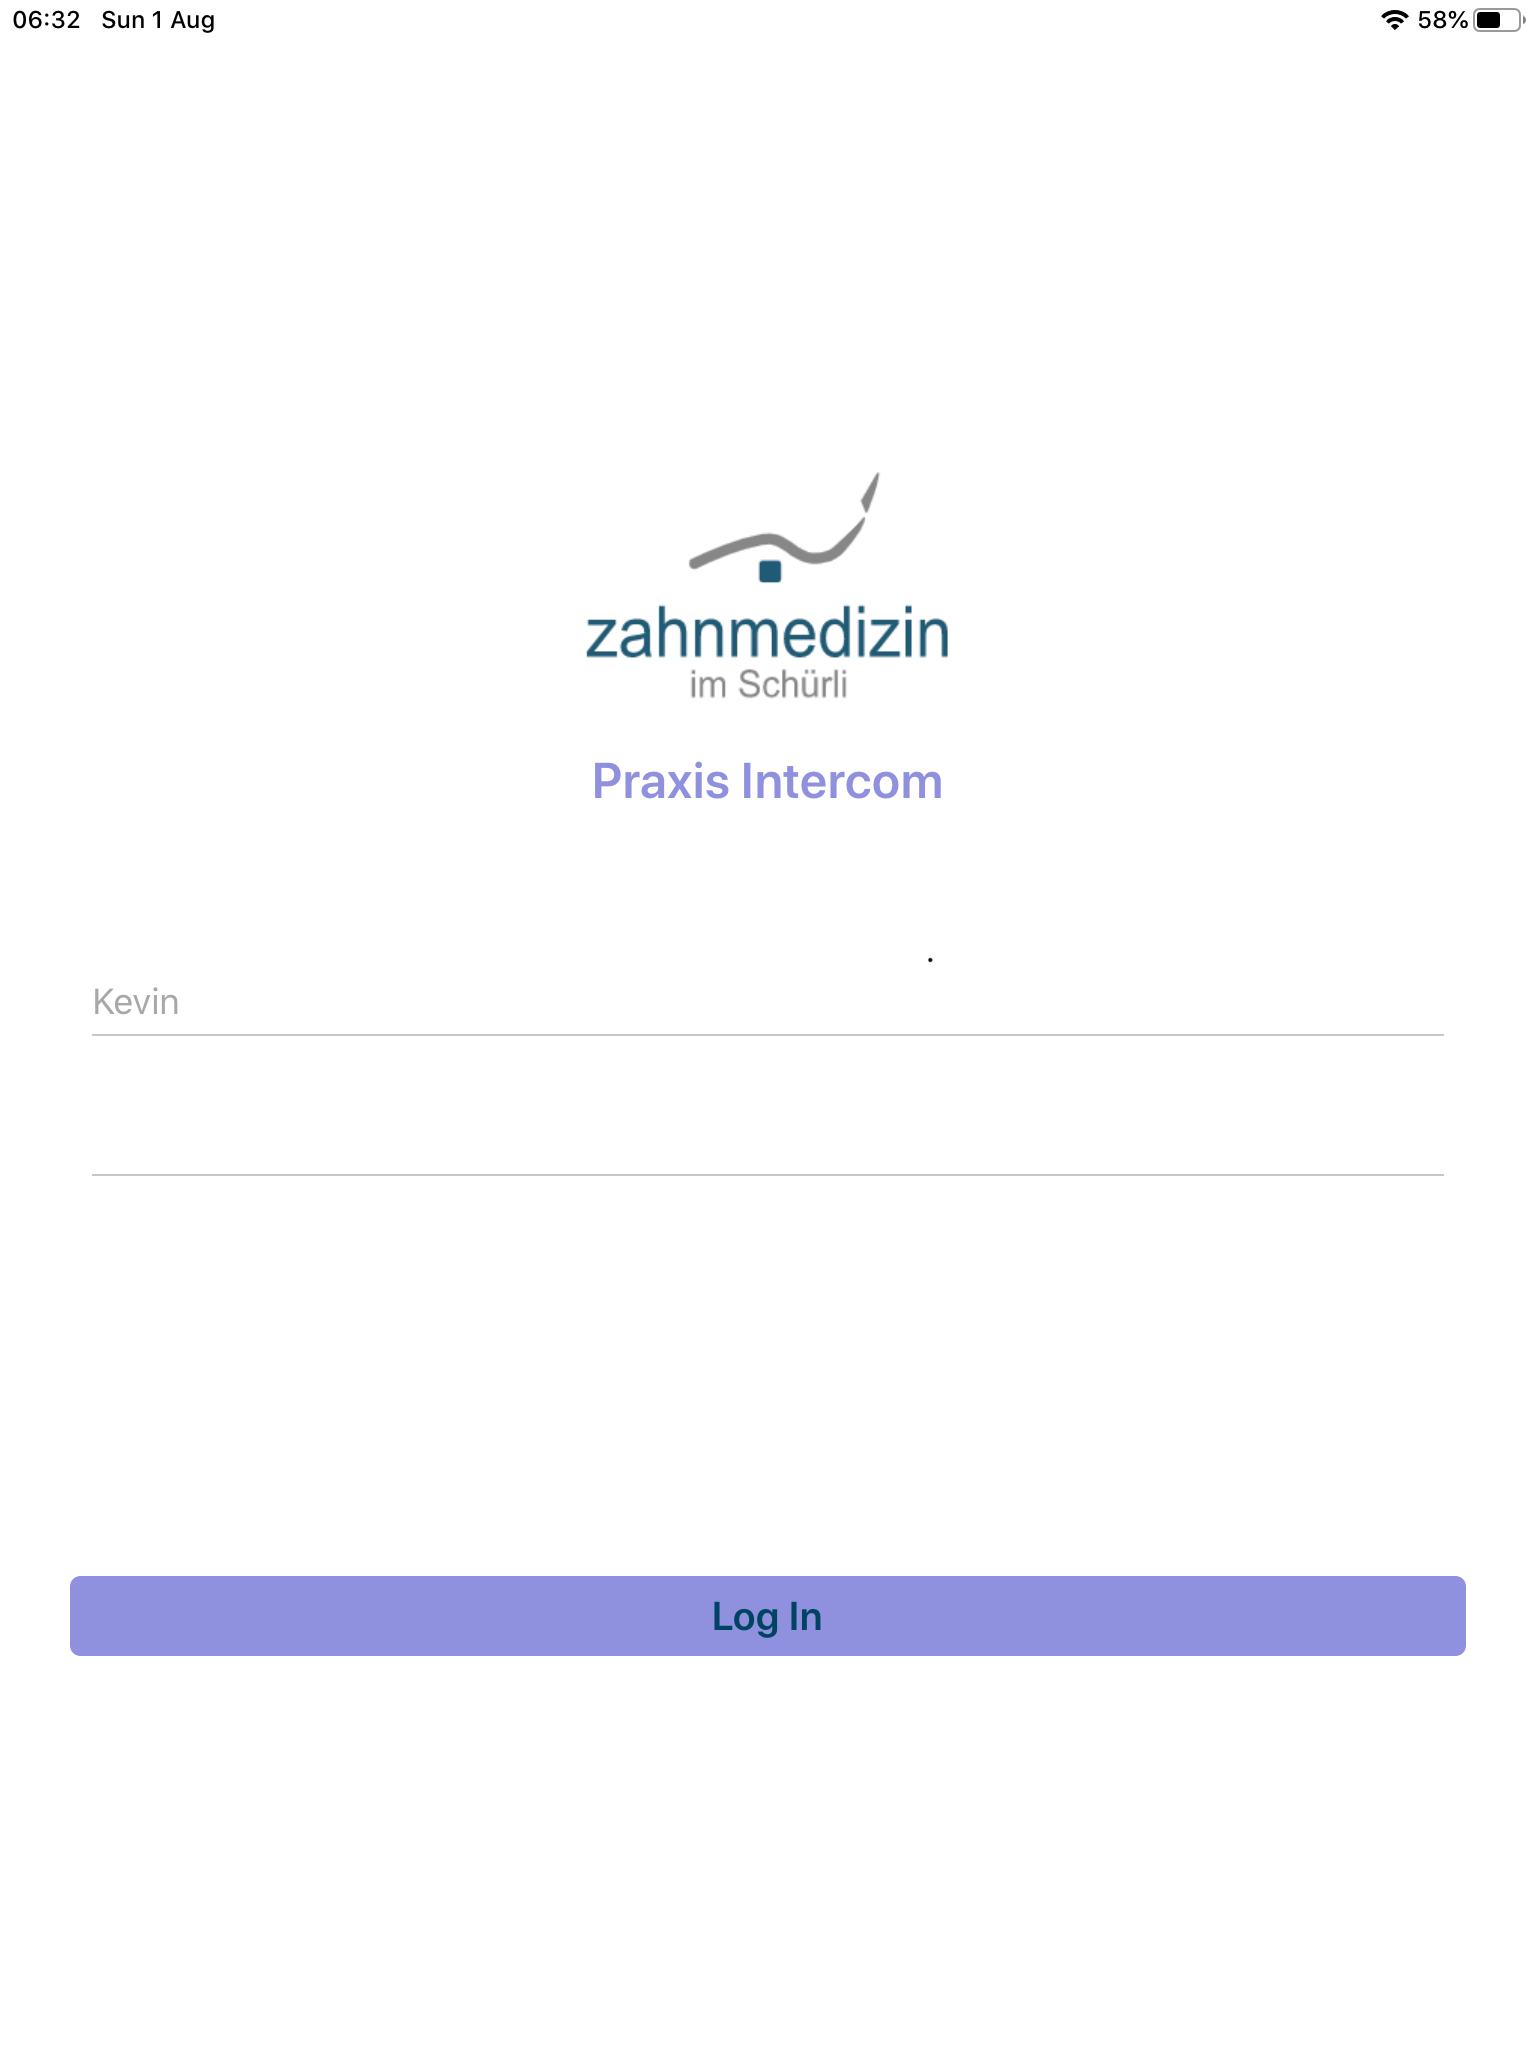
\includegraphics[width=\textwidth]{graphics/screenshot-login}
        \caption{Login}
    \end{minipage}
    \hfill
    \begin{minipage}[b]{0.4\textwidth}
        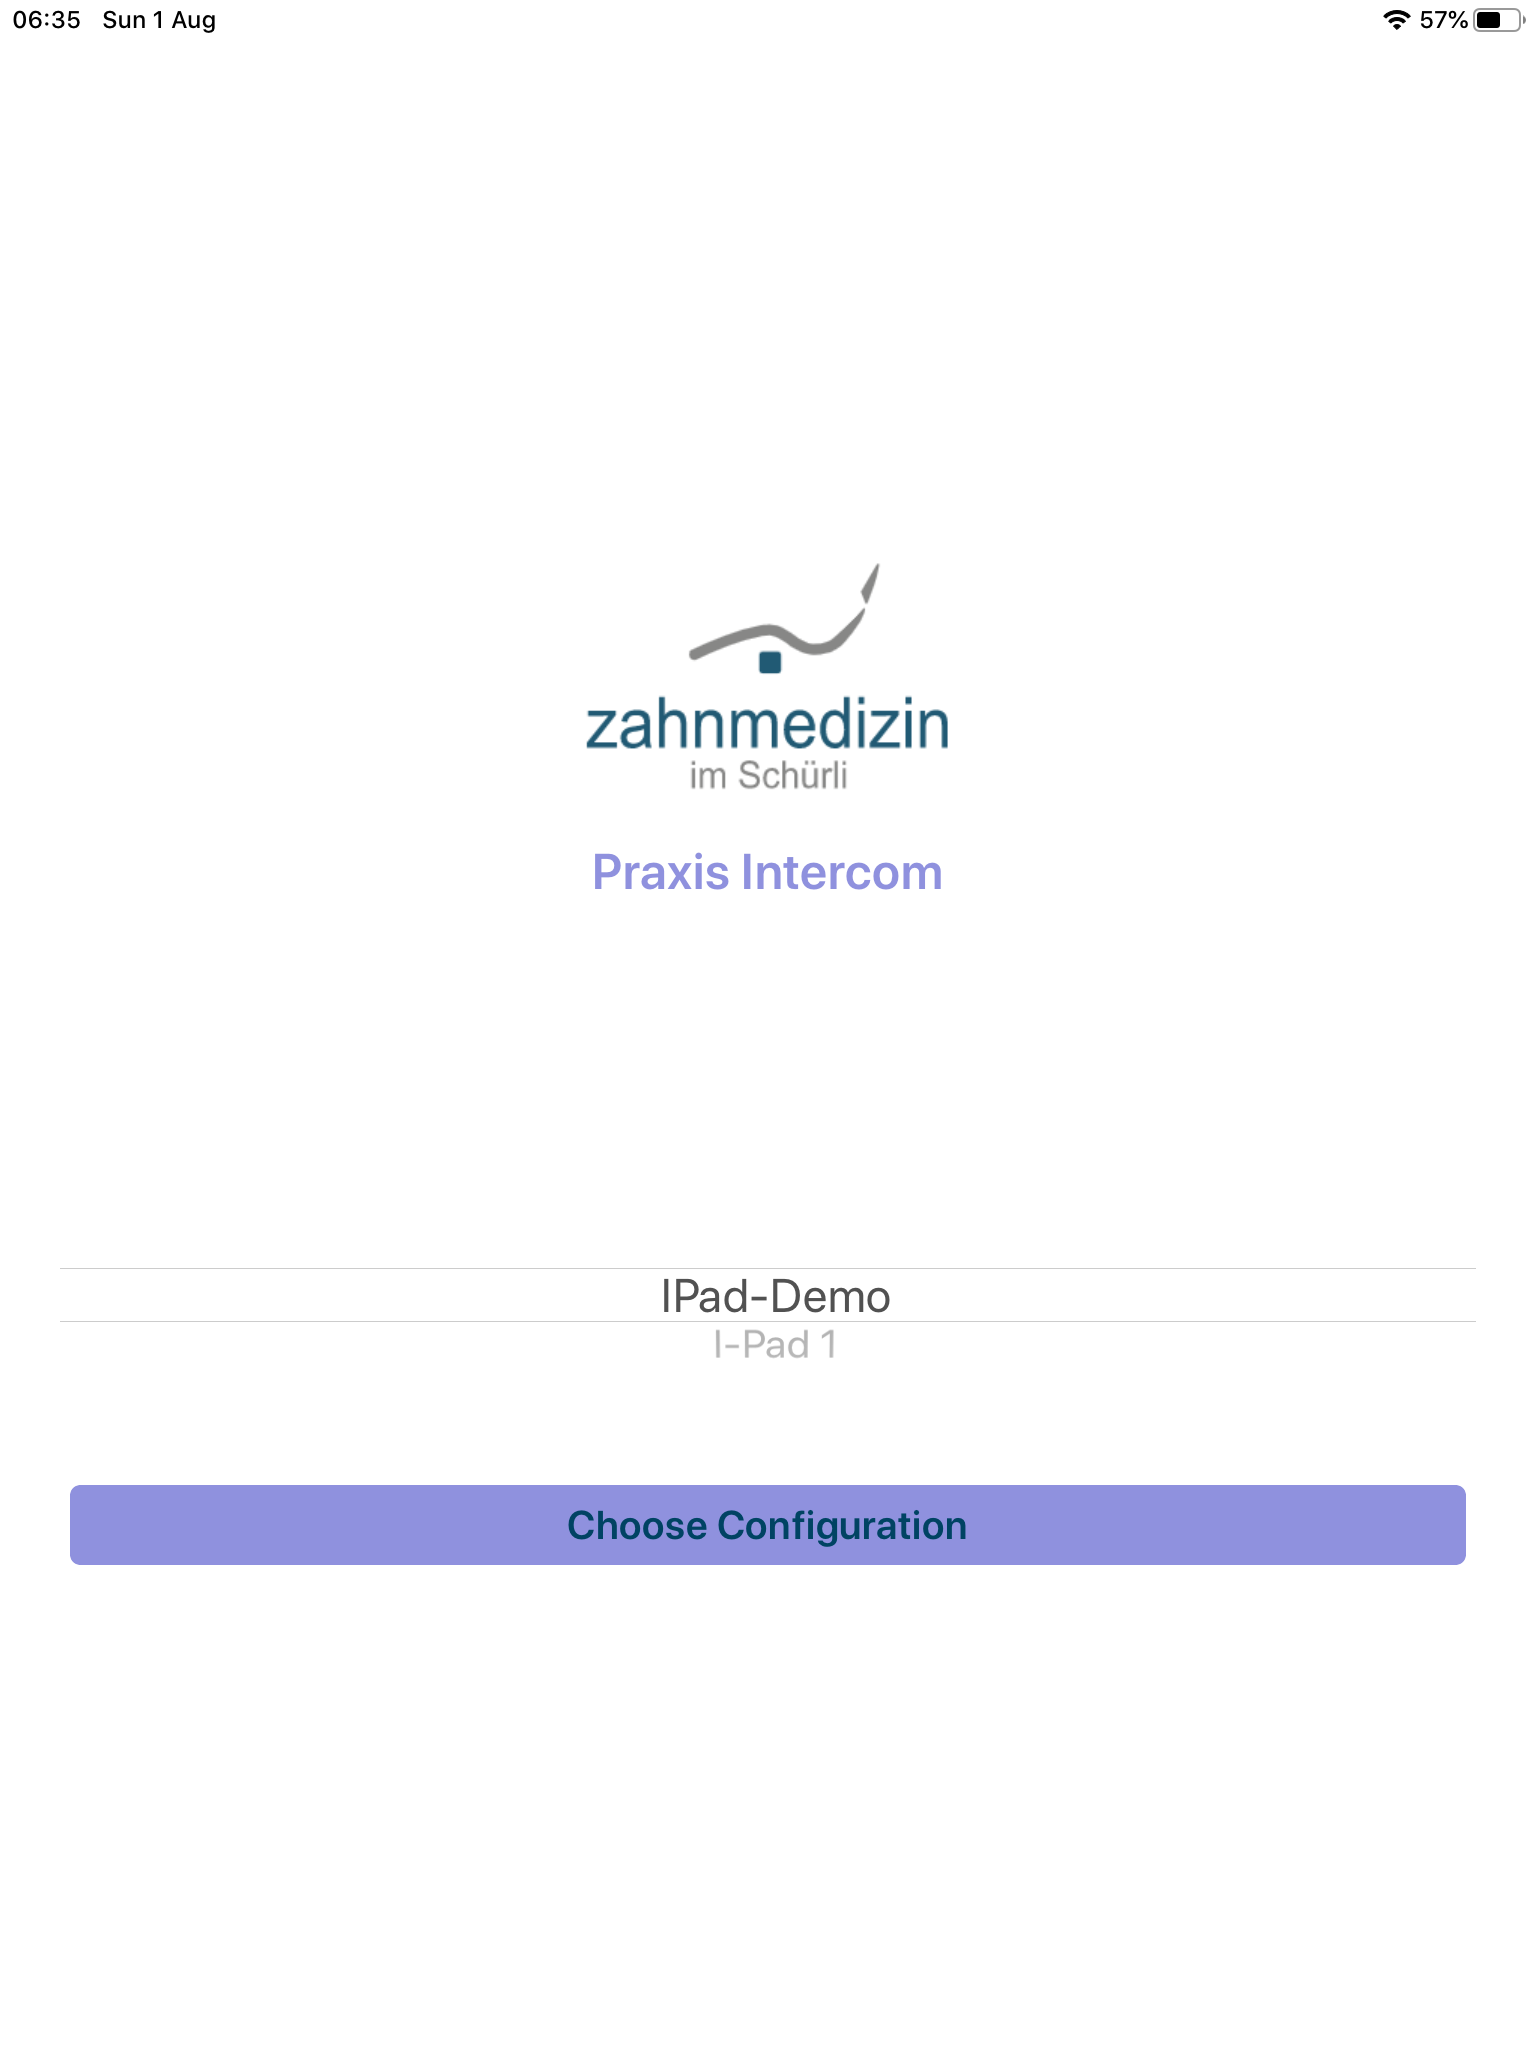
\includegraphics[width=\textwidth]{graphics/screenshots/mobileclient/screenshot-select-config}
        \caption{Konfiguration}
    \end{minipage}
    \label{fig:MobileClient-Screens1}
\end{figure}

\clearpage

Dieses Kapitel zeigt die umgesetzten Ansichten des Admin UIs.
Eine detaillierte Beschreibung, wie der Mobile Client bedient werden kann, befindet sich im Anhang der Projektdokumentation.

\begin{figure}[h]
    \centering
    \begin{minipage}[b]{0.4\textwidth}
        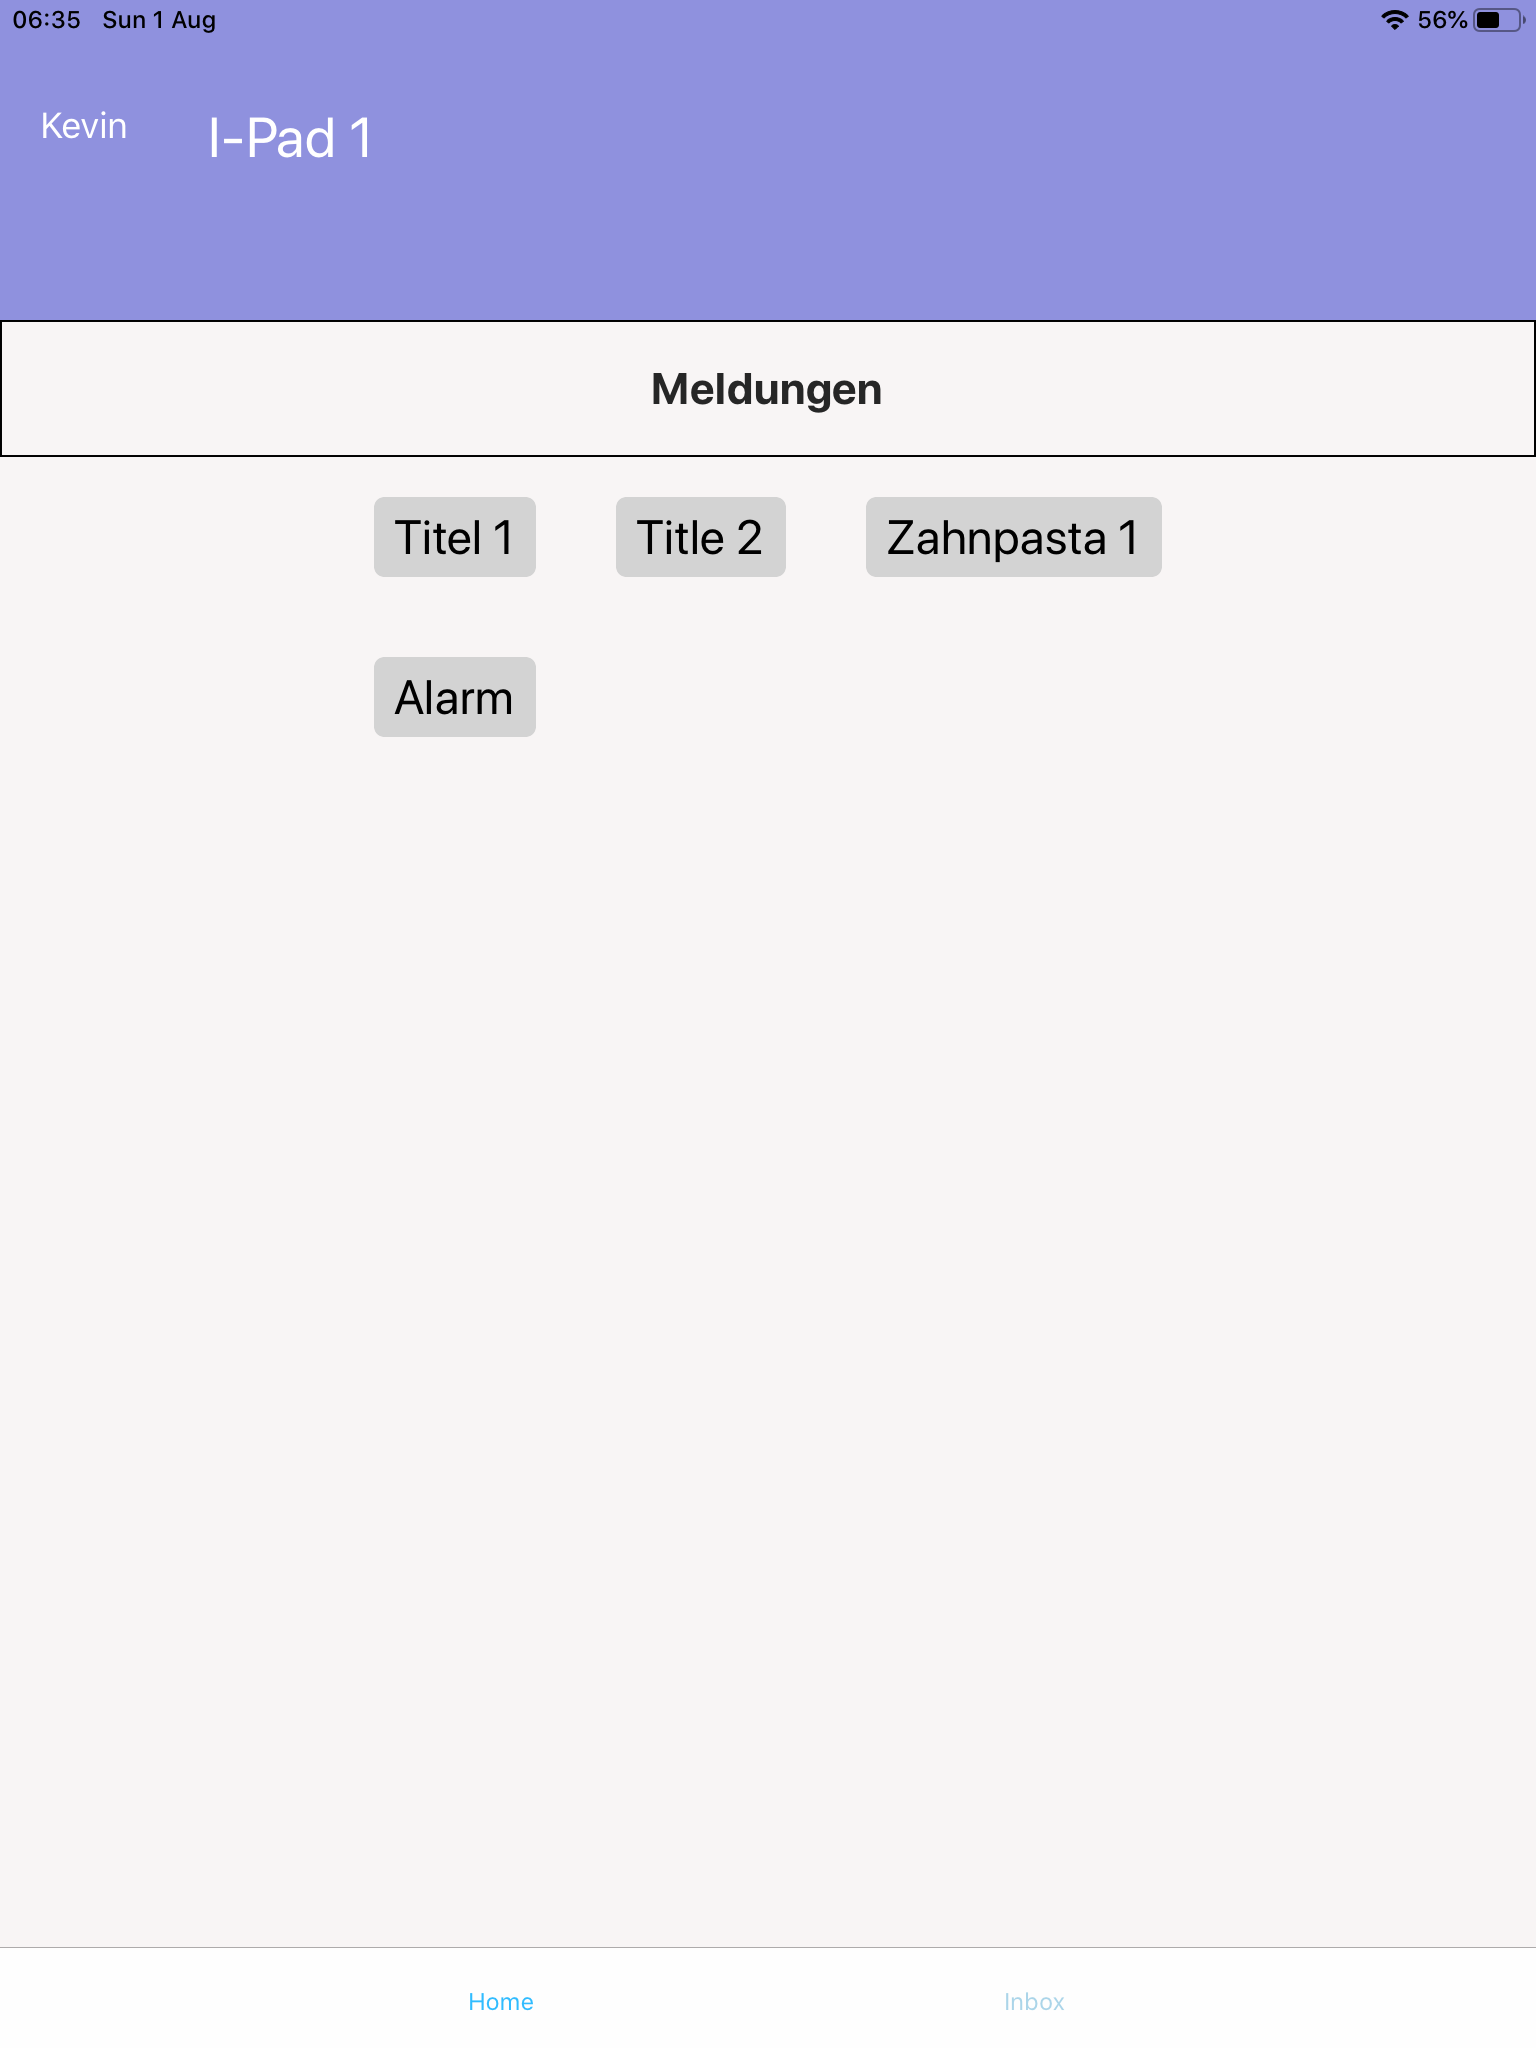
\includegraphics[width=\textwidth]{graphics/screenshots/mobileclient/screenshot-homescreen}
        \caption{Home}
    \end{minipage}
    \hfill
    \begin{minipage}[b]{0.4\textwidth}
        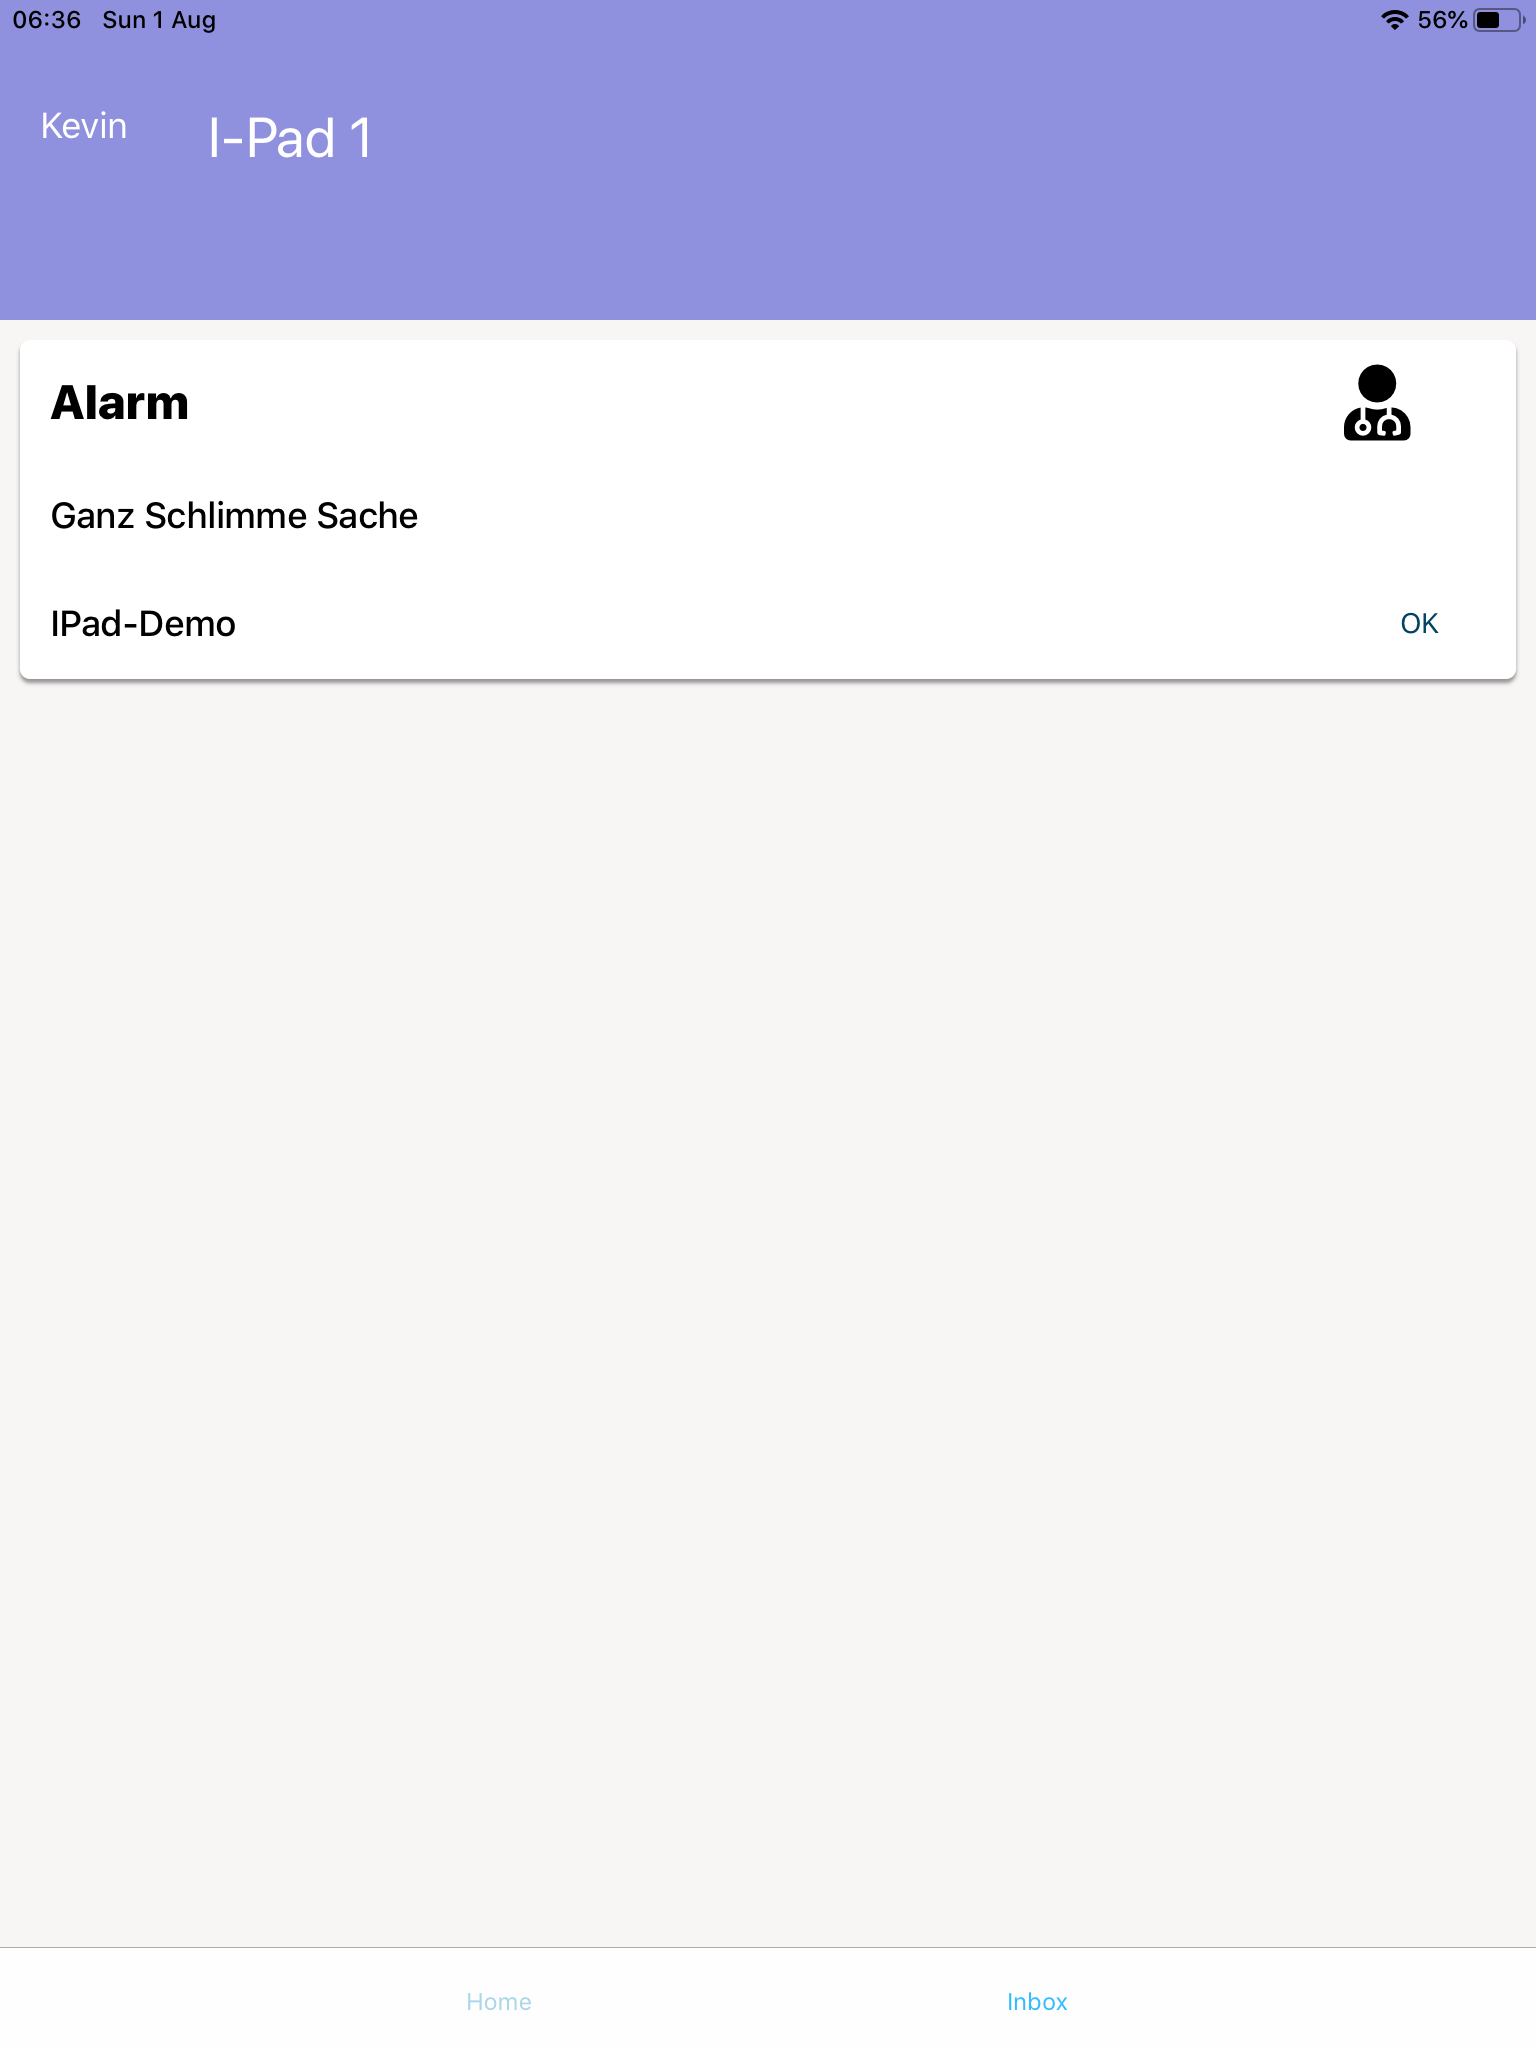
\includegraphics[width=\textwidth]{graphics/screenshots/mobileclient/screenshots-inbox}
        \caption{Inbox}
    \end{minipage}
    \label{fig:MobileClient-Screens2}
\end{figure}

\clearpage

\subsubsection{Cloud Service}

Der Cloud Service wurde wie im Konzept beschrieben umgesetzt und an den Messaging Service angebunden.

Die API ist unter www.praxisruf.ch/api erreichbar.
www.praxisruf.ch/swagger-ui.html bietet zudem zu Testzwecken die Möglichkei die Endpoints direkt anzusprechen.

\begin{minipage}[b]{1\textwidth}
    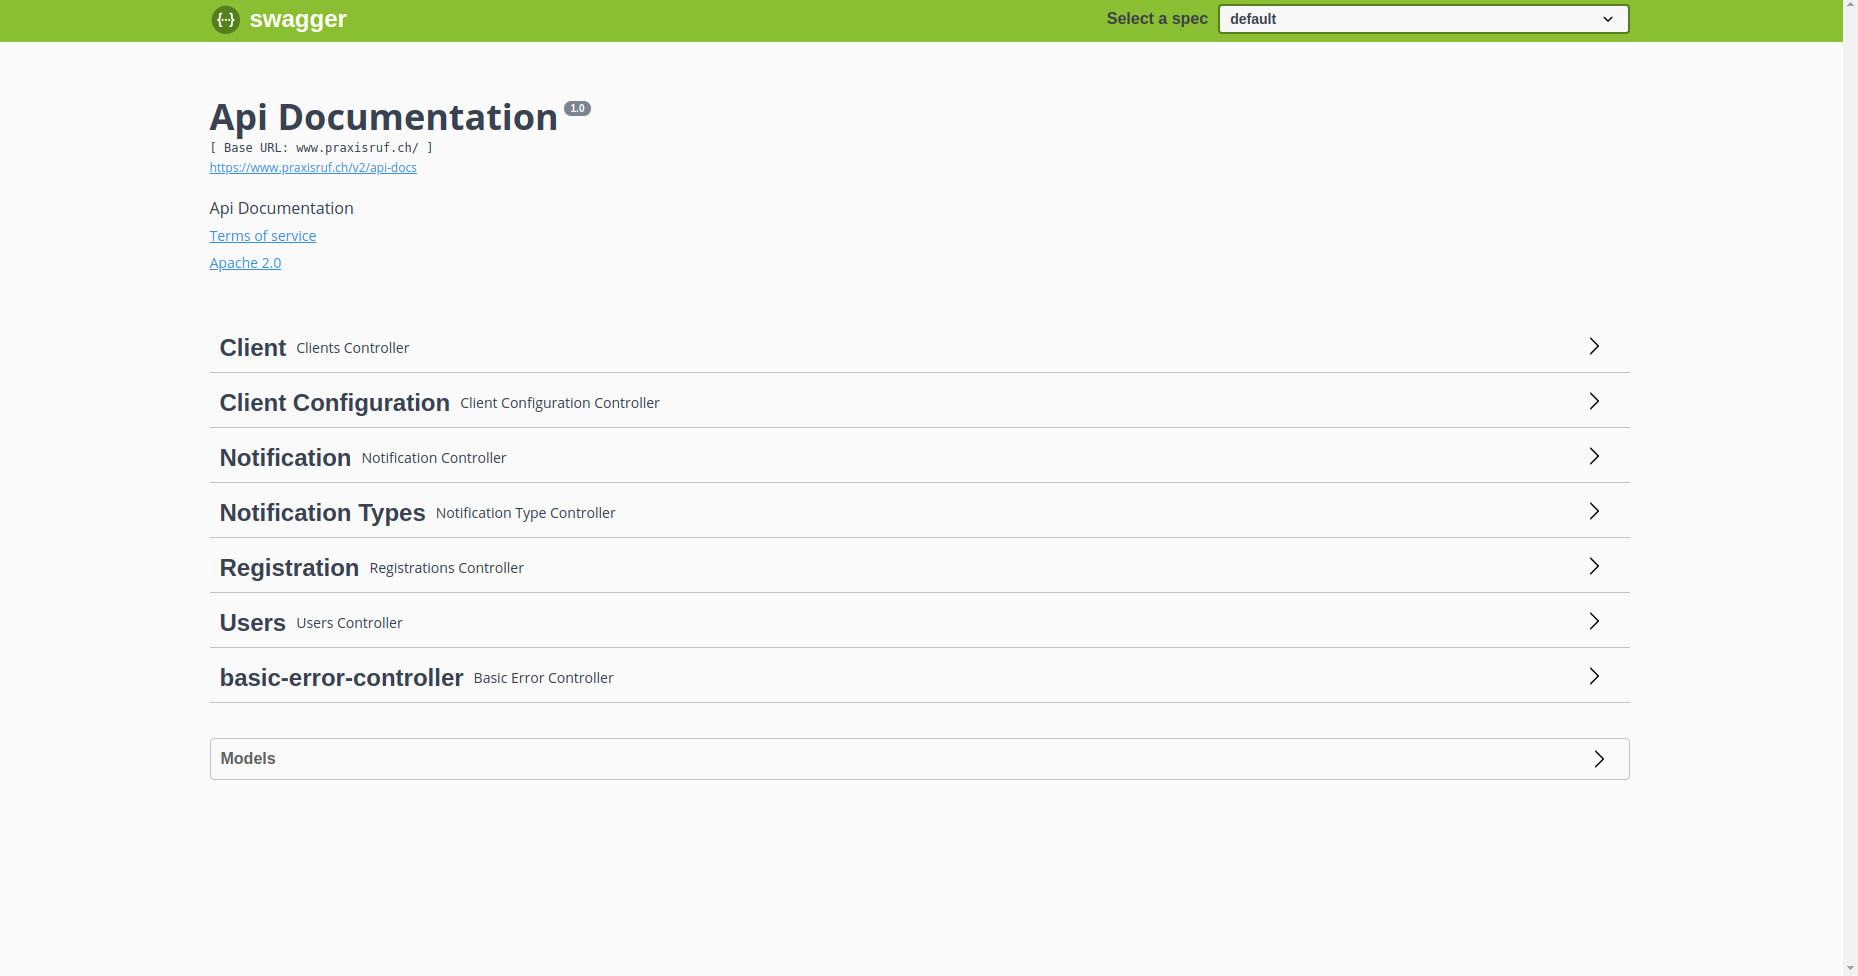
\includegraphics[width=\textwidth]{graphics/screenshots/cloud/swagger-home}
    \caption{Home}
\end{minipage}

Sorgt neben der API auch die Authentifikation die umgesetzt wurde.

\clearpage

\subsubsection{Admin UI}

\begin{figure}[h]
    \centering
    \begin{minipage}[b]{0.4\textwidth}
        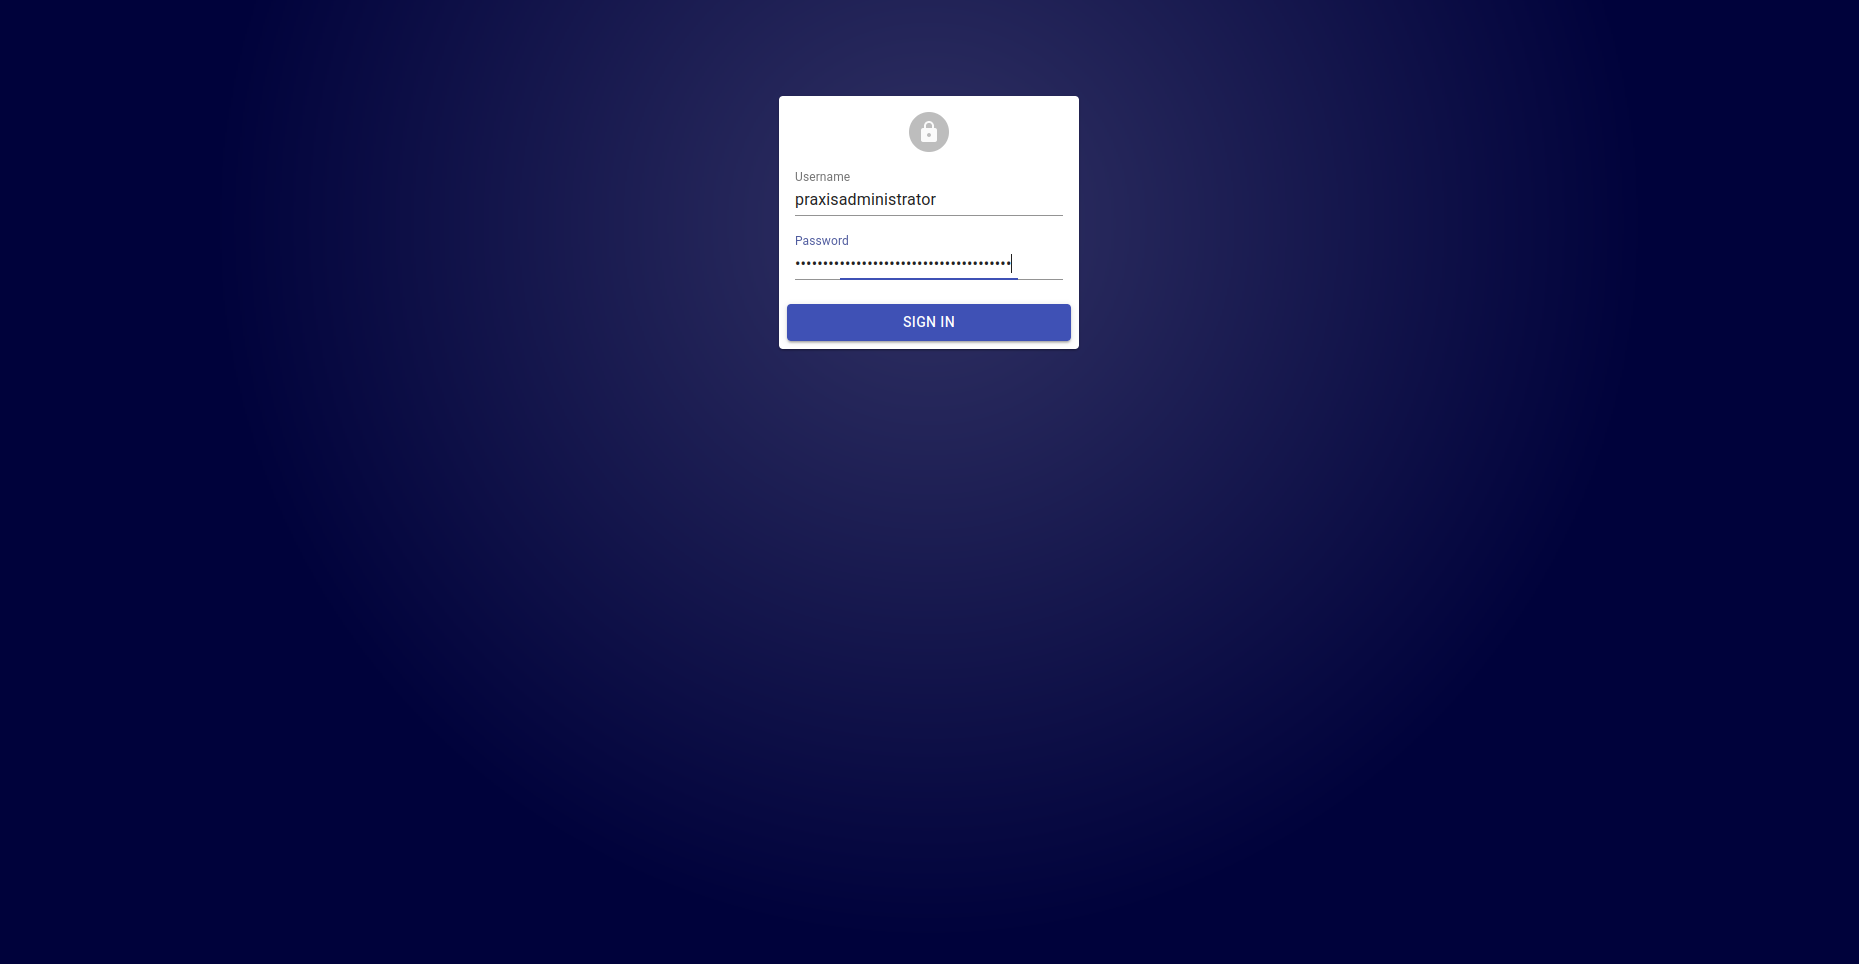
\includegraphics[width=\textwidth]{graphics/screenshots/adminui/login}
        \caption{Login}
    \end{minipage}
    \hfill
    \begin{minipage}[b]{0.4\textwidth}
        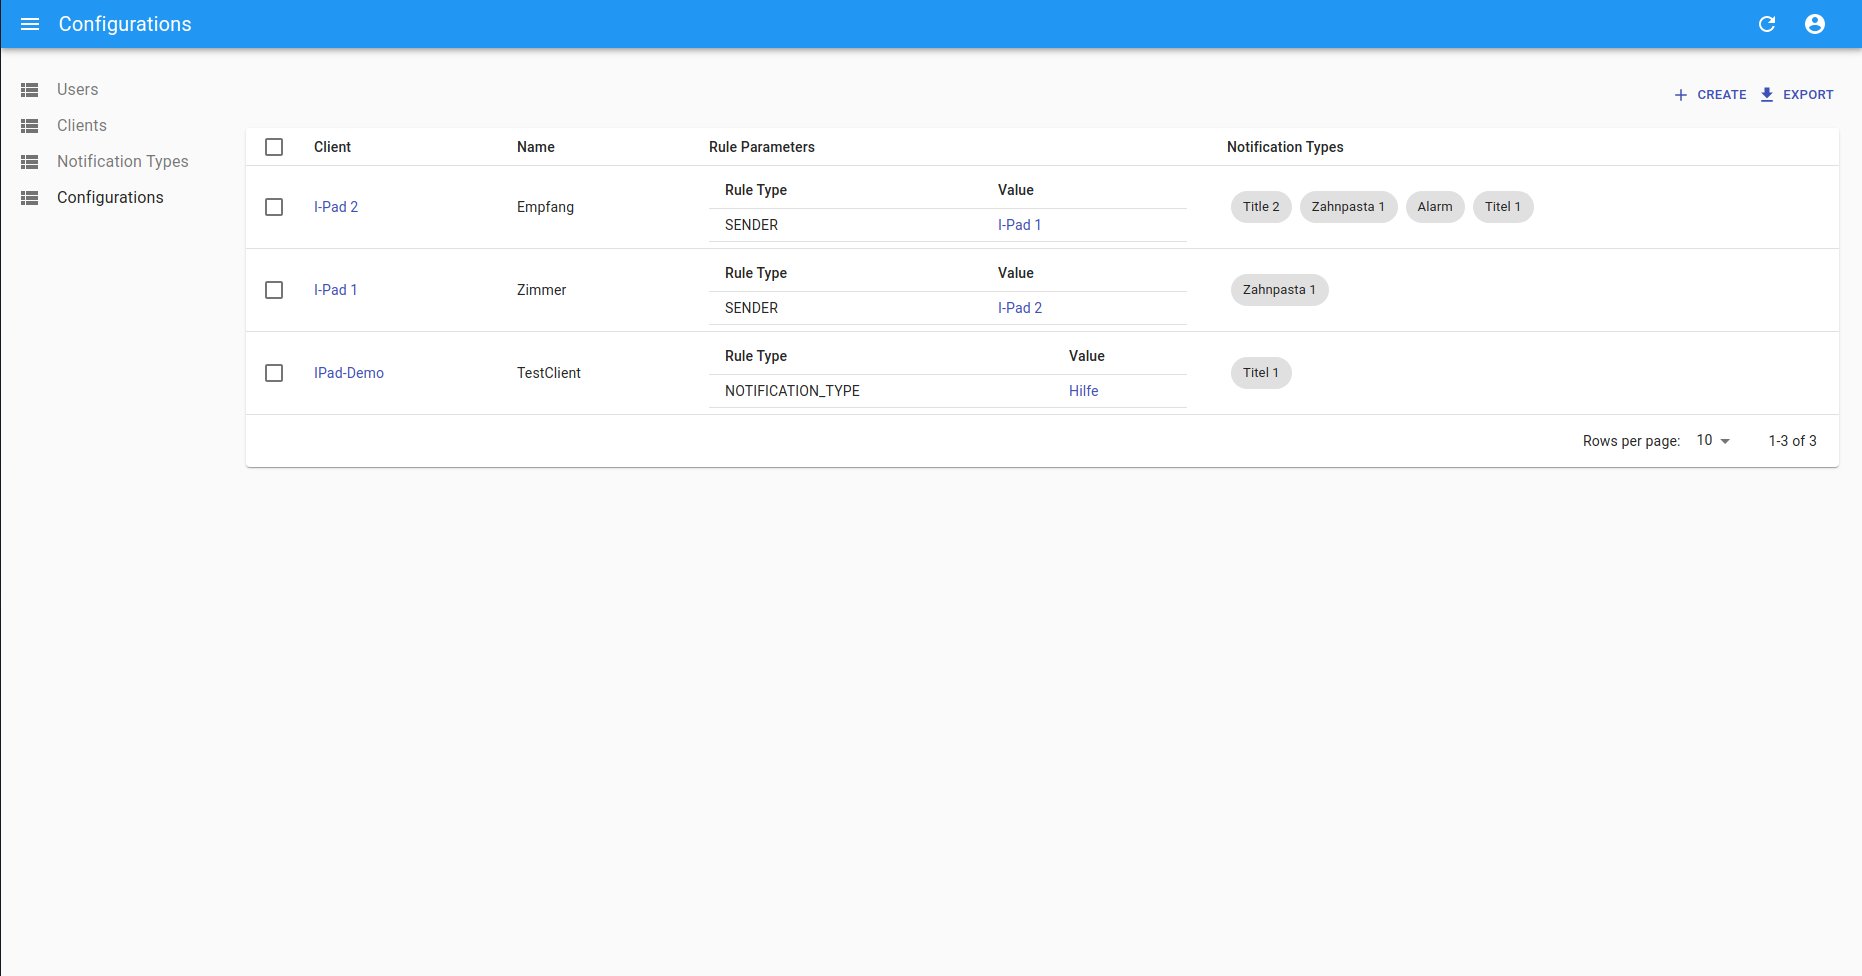
\includegraphics[width=\textwidth]{graphics/screenshots/adminui/configuration-all}
        \caption{Configuration Overview}
    \end{minipage}
    \label{fig:AdminUI-Screens1}
\end{figure}

\begin{figure}[h]
    \centering
    \begin{minipage}[b]{0.4\textwidth}
        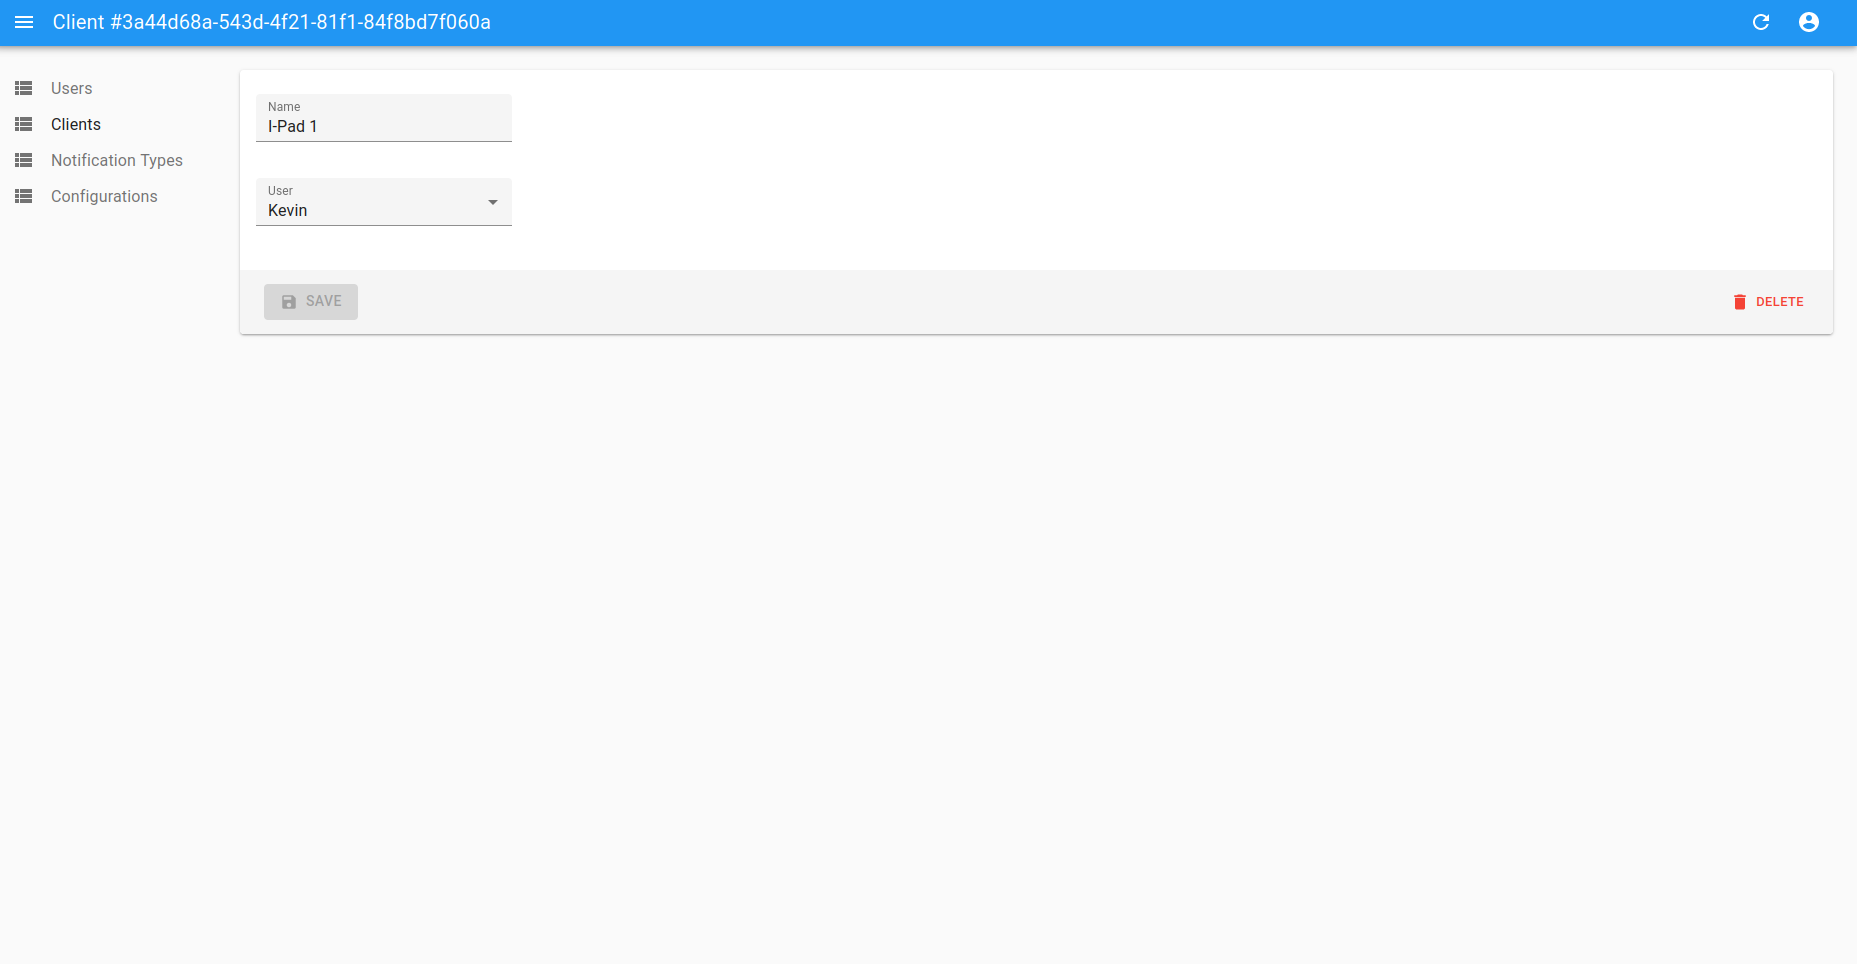
\includegraphics[width=\textwidth]{graphics/screenshots/adminui/configuration}
        \caption{Login}
    \end{minipage}
    \hfill
    \begin{minipage}[b]{0.4\textwidth}
        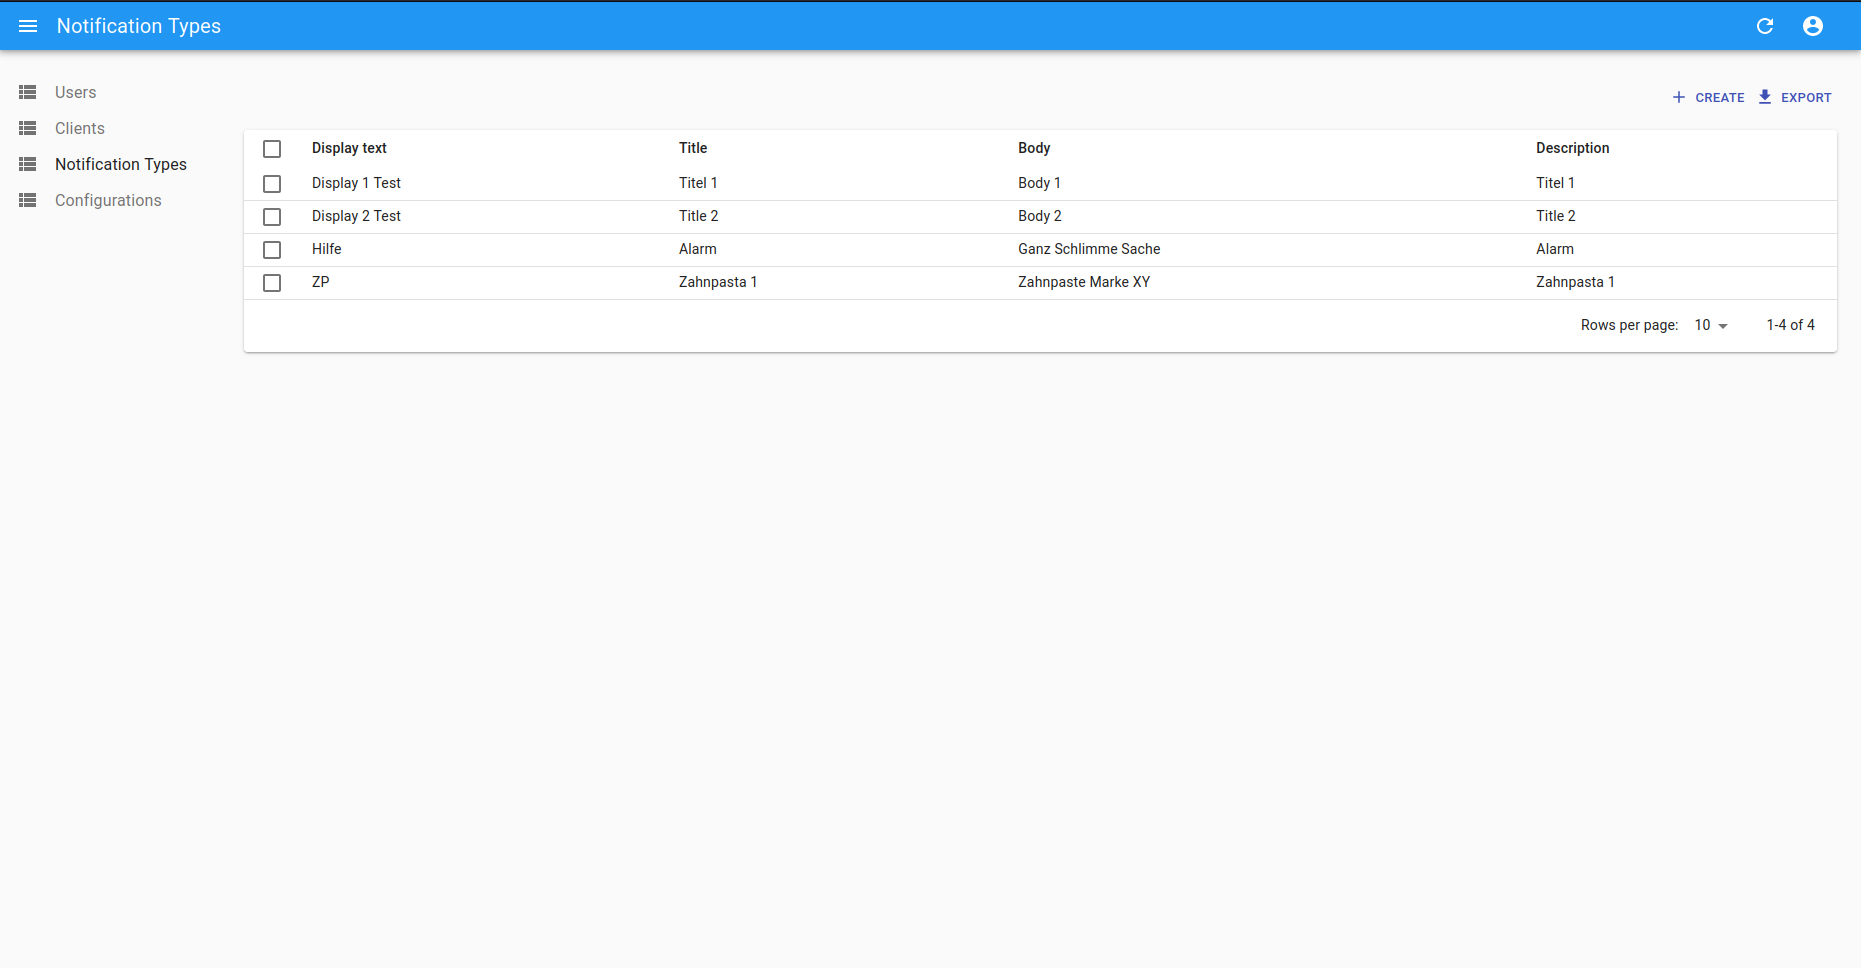
\includegraphics[width=\textwidth]{graphics/screenshots/adminui/notification-type}
        \caption{Configuration Overview}
    \end{minipage}
    \label{fig:AdminUI-Screens2}
\end{figure}




Add some screen shots

\subsection{Tests}

\subsubsection*{Benutzertests}
Wurden mit Daniel Jossen zusannem an der FH gemacht.
Mehr Tests waren wegen Ferienabwesenheiten auf Kundenseite nicht möglich.
Macht nicht so viel sinn mit nur einem Ipad.


\subsubsection*{Benutzertests}
Macht nicht so viel sinn mit nur einem Ipad.


\subsection{Herausforderungen}

Lessons learned vielleicht doch besser hier?

\begin{itemize}
    \item Dokumentation fehlt komplett in der Planung
    \item IOS Recherche viel aufwändiger als erwartet.
    \item Nativescript aufwändiger zu gebrauchen als erwartet.
    \item AWS aufsetzen ist alles andere als trivial
    \item Keine Erfahrung mit Mobile Development
    \item Stärkerer Roter Faden von Anfang an hätte geholfen
    \item Mehr testing, viel Mehr Testing.
    \item Refactoring kostet Zeit, kanns aber wert sein.
\end{itemize}







